\vspace{0.5cm} 

Chapter 3 presents the idea of several known and commonly used distributions.  R is a powerful source for accessing and using these distributions.

\section{Normal Distribution}
We have learned that the \textbf{normal distribution} can be written as 
\[ N(\mu, \sigma) \]
where $\mu$ is the mean of the distribution and $\sigma$ is the standard deviation.  Using this idea, 
we can create a standard normal distribution in one of two ways: 

\subsection{Direct Plot}
We can use a function in R called the \textit{dnorm} function which for a given posible value of the distribution, returns the probability of the distribution holding that value.  
\begin{knitrout}
\definecolor{shadecolor}{rgb}{0.969, 0.969, 0.969}\color{fgcolor}\begin{kframe}
\begin{alltt}
\hlcom{## getting a list of values to evaluate distribution}
\hlstd{X} \hlkwb{=} \hlkwd{seq}\hlstd{(}\hlopt{-}\hlnum{4}\hlstd{,} \hlnum{4}\hlstd{,} \hlnum{0.01}\hlstd{)}
\hlcom{## getting normal distribution value of the given X values }
\hlstd{Y} \hlkwb{=} \hlkwd{dnorm}\hlstd{(X,} \hlkwc{mean} \hlstd{=} \hlnum{0}\hlstd{,} \hlkwc{sd} \hlstd{=} \hlnum{1}\hlstd{)}
\hlcom{## plotting results }
\hlkwd{plot}\hlstd{(X,Y,} \hlkwc{type} \hlstd{=} \hlstr{"l"}\hlstd{)}
\end{alltt}
\end{kframe}

{\centering 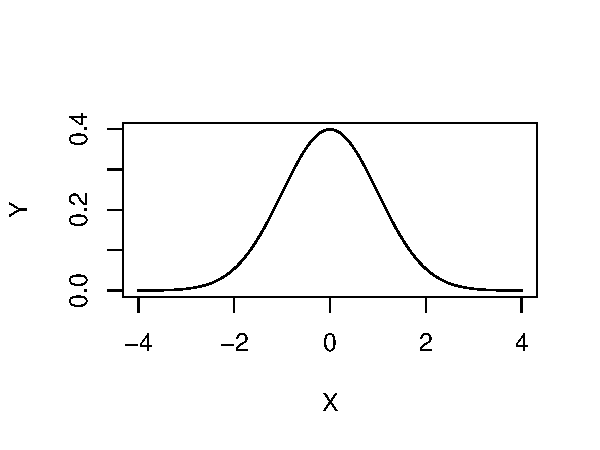
\includegraphics[width=\maxwidth]{figure/unnamed-chunk-1-1} 

}



\end{knitrout}

\subsection{Through Simulation}
The second method involves sampling randomly from the known normal distribution to simulate the probabilities that we drew directly in the above method.  In this case, we use the function \textit{rnorm}, which takes $n$ number of random samples from the normal distribution with the given mean and standard deviation.  In the \textit{hist} command, we include the specification that \textit{freq = FALSE} to make the plot reflect percentages rather than frequency counts.  
\begin{knitrout}
\definecolor{shadecolor}{rgb}{0.969, 0.969, 0.969}\color{fgcolor}\begin{kframe}
\begin{alltt}
\hlkwd{set.seed}\hlstd{(}\hlnum{1}\hlstd{)}
\hlstd{x} \hlkwb{<-} \hlkwd{rnorm}\hlstd{(}\hlkwc{n} \hlstd{=} \hlnum{100000}\hlstd{,} \hlkwc{mean} \hlstd{=} \hlnum{0}\hlstd{,} \hlkwc{sd} \hlstd{=} \hlnum{1}\hlstd{)}
\hlkwd{hist}\hlstd{(x,} \hlkwc{breaks} \hlstd{=} \hlnum{100}\hlstd{,} \hlkwc{freq} \hlstd{=} \hlnum{FALSE}\hlstd{)}
\end{alltt}
\end{kframe}

{\centering 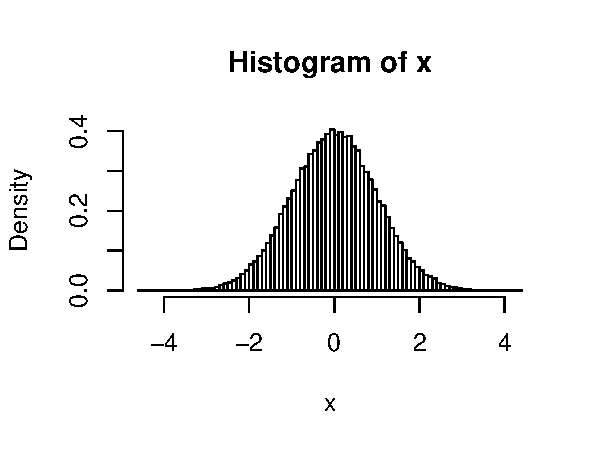
\includegraphics[width=\maxwidth]{figure/unnamed-chunk-2-1} 

}



\end{knitrout}

\subsection{A Comparison} 
To see how comparable the two methods are, we can plot them on the same graph as follows.  
\begin{knitrout}
\definecolor{shadecolor}{rgb}{0.969, 0.969, 0.969}\color{fgcolor}\begin{kframe}
\begin{alltt}
\hlkwd{hist}\hlstd{(x,} \hlkwc{freq} \hlstd{=} \hlnum{FALSE}\hlstd{,} \hlkwc{breaks} \hlstd{=} \hlnum{100}\hlstd{)}
\hlkwd{lines}\hlstd{(X,Y,} \hlkwc{col} \hlstd{=} \hlstr{"red"}\hlstd{)}
\end{alltt}
\end{kframe}

{\centering 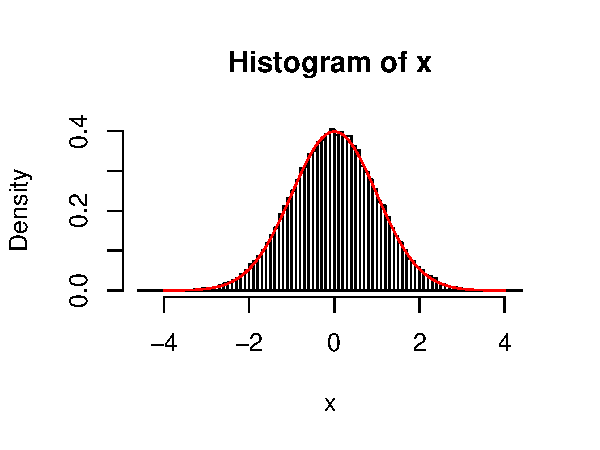
\includegraphics[width=\maxwidth]{figure/unnamed-chunk-3-1} 

}



\end{knitrout}
Note that the two show very similar results.  For practical purposes, we typically use \textit{dnorm} as it only requires one command and is the asymptotic result of simulations, rather than an approximation.  

\subsection{Probability Functions}
For the normal distribution, there are two more functions that are very useful, \textit{pnorm} and \textit{qnorm}. 

\subsubsection{pnorm} 
The function \textit{pnorm} tells you the percentage of the normal distribution that is less than or equal to the value you put in.  This corresponds to the gray area in the below plot and can be written as $pnorm(x, mean = \mu, sd = \sigma)$ which is equivalent to $P(X < x)$ where $X \sim N(\mu, \sigma)$ and $x$ is the point of interest.    
 
\begin{knitrout}
\definecolor{shadecolor}{rgb}{0.969, 0.969, 0.969}\color{fgcolor}

{\centering 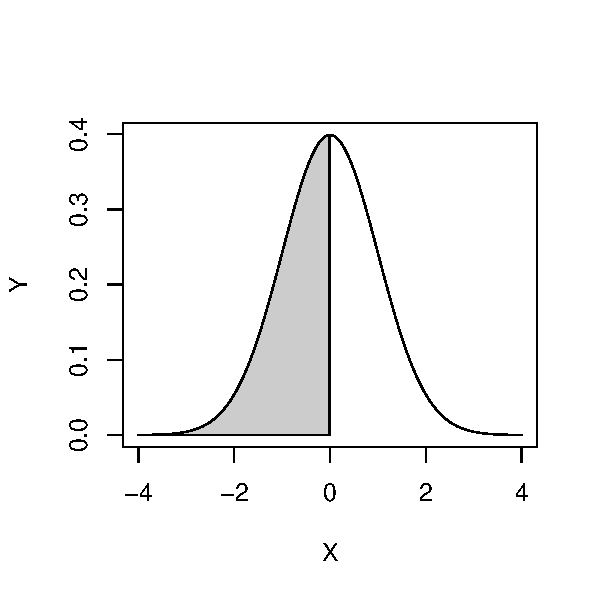
\includegraphics[width=\maxwidth]{figure/unnamed-chunk-4-1} 

}



\end{knitrout}

For some example scenarios, where we want to find a proportion of the normal distribution given $x$ or $z$, we can use the following configurations of \textit{pnorm()}: 
\begin{itemize}
\item $pnorm(z) = P(Z \leq z)$ 
\item $pnorm(z, lower.tail = FALSE) = P(Z > z)$ 
\item $pnorm(x, \mu, \sigma) = P(X \leq x)$ where $X = \sigma Z + \mu$ 
\item $pnorm(x, \mu, \sigma, lower.tail = FALSE) = P(X > x)$ where $X = \sigma Z + \mu$ 
\end{itemize}

\subsubsection{qnorm} 
On the other hand, the \textit{qnorm} function is the inverse function, instead giving the $X$ value such that the given percentage of the distribution is less than or equal to that value. This function takes a known probability and returns a value on the normal distribution that is corresponding.  

Some sample configurations of using \textit{qnorm()} can be as follows,  
\begin{itemize}
\item $qnorm(p) = P(Z \leq z)$ 
\item $qnorm(p, lower.tail = FALSE) = P(Z > z)$ 
\item $qnorm(p, \mu, \sigma) = P(X \leq x)$ where $X = \sigma Z + \mu$ 
\item $qnorm(p, \mu, \sigma, lower.tail = FALSE) = P(X > x)$ where $X = \sigma Z + \mu$ 
\end{itemize}

\section{Binomial Distribution}
We can write a random variable which follows a binomial distribution as
\[ X \sim Binom(n,p) \]
where $n$ represents the sample size and $p$ represents the probability of success.  

The functions we saw above for the normal distribution can be similarly used for the \textbf{binomial distribution} as follows where the necessary arguments are \textit{size} and \textit{prob}, corresponding respectively to $n$ and $p$ in our above representation of the binomial.
\begin{itemize} 
\item \textit{dbinom}
\item \textit{rbinom}
\item \textit{pbinom}
\item \textit{qbinom}
\end{itemize}

Similar to the above example with the normal distribution, we can use these functions in multiple ways to work with the binomial distribution.  

\subsection{Accessing the Binomial Distribution}
As we did above, we can directly access the binomial distribution using the \textit{dbinom} function as follows: 
\begin{knitrout}
\definecolor{shadecolor}{rgb}{0.969, 0.969, 0.969}\color{fgcolor}\begin{kframe}
\begin{alltt}
\hlcom{## Splitting the graphics window into two panes }
\hlkwd{par}\hlstd{(}\hlkwc{mfrow}\hlstd{=}\hlkwd{c}\hlstd{(}\hlnum{1}\hlstd{,}\hlnum{2}\hlstd{))}
\hlcom{## Directly plotting the binomial distribution}
 \hlcom{# getting a list of values to evaluate distribution}
\hlstd{X} \hlkwb{=} \hlkwd{seq}\hlstd{(}\hlnum{0}\hlstd{,} \hlnum{10}\hlstd{,} \hlnum{1}\hlstd{)}
 \hlcom{# getting normal distribution value of the given X values }
\hlstd{Y} \hlkwb{=} \hlkwd{dbinom}\hlstd{(X,} \hlkwc{size} \hlstd{=} \hlnum{10}\hlstd{,} \hlkwc{prob} \hlstd{=} \hlnum{.25}\hlstd{)}
 \hlcom{# plotting results }
\hlkwd{plot}\hlstd{(X,Y,} \hlkwc{type} \hlstd{=} \hlstr{"s"}\hlstd{,} \hlkwc{main} \hlstd{=} \hlstr{"Direct Plot"}\hlstd{,} \hlkwc{xlim} \hlstd{=} \hlkwd{c}\hlstd{(}\hlnum{0}\hlstd{,}\hlnum{10}\hlstd{))}

\hlcom{## Instead Using Simulation}
\hlkwd{set.seed}\hlstd{(}\hlnum{1}\hlstd{)}
\hlstd{x} \hlkwb{<-} \hlkwd{rbinom}\hlstd{(}\hlkwc{n} \hlstd{=} \hlnum{100000}\hlstd{,} \hlkwc{size} \hlstd{=} \hlnum{10}\hlstd{,} \hlkwc{prob} \hlstd{=} \hlnum{.25}\hlstd{)}
\hlkwd{hist}\hlstd{(x,} \hlkwc{breaks} \hlstd{=} \hlnum{10}\hlstd{,} \hlkwc{freq} \hlstd{=} \hlnum{FALSE}\hlstd{,}\hlkwc{right} \hlstd{=} \hlnum{FALSE}\hlstd{,} \hlkwc{main} \hlstd{=} \hlstr{"Simulation"}\hlstd{,} \hlkwc{xlim} \hlstd{=} \hlkwd{c}\hlstd{(}\hlnum{0}\hlstd{,}\hlnum{10}\hlstd{))}
\hlkwd{box}\hlstd{()}
\end{alltt}
\end{kframe}

{\centering 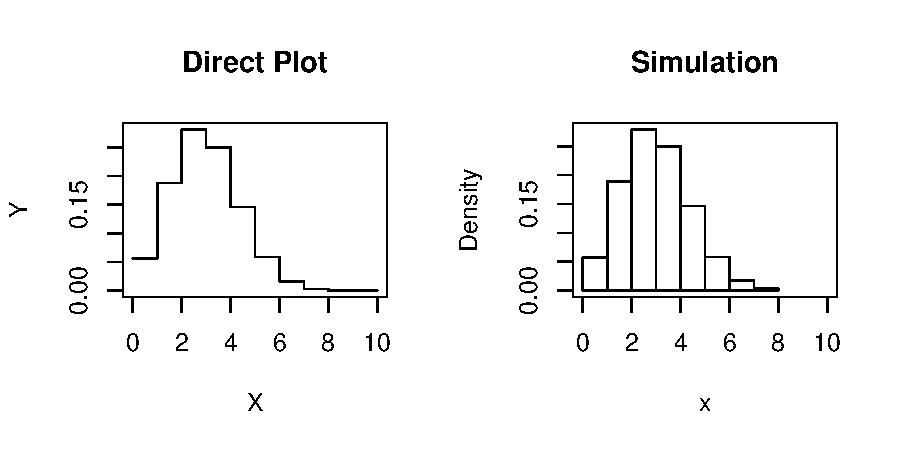
\includegraphics[width=\maxwidth]{figure/unnamed-chunk-5-1} 

}



\end{knitrout}

\subsection{Comparison of the Methods}
Instead of side by side, we can superimpose the two graphs for direct comparison.  
\begin{knitrout}
\definecolor{shadecolor}{rgb}{0.969, 0.969, 0.969}\color{fgcolor}\begin{kframe}
\begin{alltt}
\hlkwd{hist}\hlstd{(x,} \hlkwc{breaks} \hlstd{=} \hlnum{10}\hlstd{,} \hlkwc{freq} \hlstd{=} \hlnum{FALSE}\hlstd{,}\hlkwc{right} \hlstd{=} \hlnum{FALSE}\hlstd{)}
\hlkwd{lines}\hlstd{(X,Y,} \hlkwc{type} \hlstd{=} \hlstr{"s"}\hlstd{,} \hlkwc{col} \hlstd{=} \hlstr{"red"}\hlstd{)}
\end{alltt}
\end{kframe}

{\centering 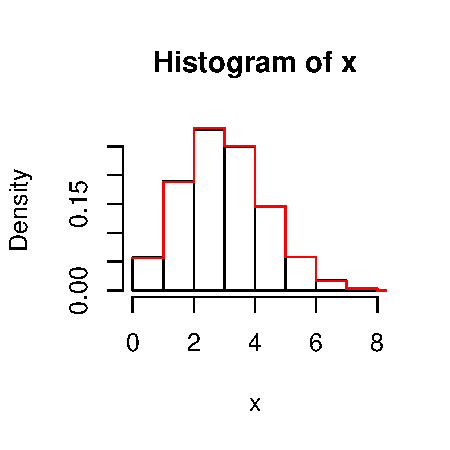
\includegraphics[width=\maxwidth]{figure/unnamed-chunk-6-1} 

}



\end{knitrout}

\section{Continuous and Discrete Distributions}
Using the binomial distribution highlights an important feature of distributions that we must consider: whether the random variable is \textbf{discrete} or \textbf{continuous}.  A discrete distribution can only take on specified values, typically the integers. The binomial is a great example of this - it can be any integer greater than or equal to zero.  For example, the possible values of a binomial are \{0, 1, 2, 3, ...\}.  

On the other hand, a continuous distribution can take on any real number within a specified range.  For example, looking at the standard normal distribution, a list of some possible values could be \{0, 0.1, 0.01, 0.001, 0.0001, ...\}.  This is a limited list of the infinite list of possible values that a continuous distribution could take on.  

The reason we care about the classification of a random variable as discrete or continous is that it affects how we use our probability functions in $R$.  Let's walk through an example to see the difference.  Suppose we have a normally distributed random variable, $X$, and a binomially distributed random variable, $Y$. 
\[ X \sim N(0,1) \; \; \; \; \; \; \; \; \; \; \; \;  Y \sim Binom(1,0.5) \]
If we wanted to know for these two distributions, the probability of being less than 2, we would consider $P(X < 2)$ and $P(Y < 2)$.  However, for the binomial distribution $P(Y<2) = P(Y \leq 1) = P(Y=0) + P(Y=1)$ because there is a discrete set of possible values that $Y$ can take on.  $Y$ cannot take on any non-integer value between 0 and 2, whereas the normal distribution can take on any of those values.  On the other hand, for the normal distribution, solving for $P(Y<2)$ is mathematically equivalent to $P(Y \leq 2)$.  

So to solve for these probabilities, we would use \textit{pnorm} and \textit{pbinom}, but we have to be careful with the discrete binomial case because these functions automatically give the less than or equal to probability, not just the less than probability.  The correct commands to use would be 
\begin{knitrout}
\definecolor{shadecolor}{rgb}{0.969, 0.969, 0.969}\color{fgcolor}\begin{kframe}
\begin{alltt}
\hlkwd{pnorm}\hlstd{(}\hlnum{2}\hlstd{)}
\end{alltt}
\begin{verbatim}
## [1] 0.9772499
\end{verbatim}
\begin{alltt}
\hlkwd{pbinom}\hlstd{(}\hlnum{1}\hlstd{,} \hlkwc{size} \hlstd{=} \hlnum{15}\hlstd{,} \hlkwc{prob}\hlstd{=}\hlnum{0.5}\hlstd{)}
\end{alltt}
\begin{verbatim}
## [1] 0.0004882812
\end{verbatim}
\end{kframe}
\end{knitrout}

To summarize, we would use the binomial probaility functions as follows, 
\begin{itemize} 
\item $dbinom(x,n,p) = P(X = x)$ 
\item $pbinom(x,n,p) = P(X \leq x)$ 
\item $pbinom(x,n,p, lower.tail = FALSE) = P(X > x)$ 
\end{itemize} 


\section{Poisson Distribution}
Similarly, we can build out the functions for the \textbf{poisson distribution} as the following where the necessary argument is \textit{lambda}
\begin{itemize} 
\item \textit{dbinom}
\item \textit{rbinom}
\item \textit{pbinom}
\item \textit{qbinom}
\end{itemize}

\section{Geometric Distribution}
We can follow the same pattern for the \textbf{geometric distribution} to get the following where the necessary argument is \textit{prob}
\begin{itemize} 
\item \textit{dgeom}
\item \textit{rgeom}
\item \textit{pgeom}
\item \textit{qgeom}
\end{itemize}

\section{Negative Binomial Distribution}
Finally, we can follow the same pattern for the \textbf{negative binomial distribution} to get the following where the necessary arguments are \textit{prob} and \textit{size}
\begin{itemize} 
\item \textit{dnbinom}
\item \textit{rnbinom}
\item \textit{pnbinom}
\item \textit{qnbinom}
\end{itemize}


